\documentclass[14pt]{extarticle}
\def\activityid{F09-K-v3}\usepackage[letterpaper,margin=.65in,top=.60in,bottom=.65in]{geometry}
\usepackage[T1]{fontenc}
\usepackage[default]{sourcesanspro}
\usepackage{microtype,tikz,array,tabularx,fancyhdr,amsmath,amssymb}
\usepackage[hidelinks]{hyperref}
\usetikzlibrary{calc,arrows.meta}
\setlength{\parindent}{0pt}\setlength{\parskip}{7pt}
\setlength{\headheight}{0pt}\setlength{\footskip}{26pt}\setlength{\emergencystretch}{2em}
\pagestyle{fancy}\fancyhf{}\renewcommand{\headrulewidth}{0pt}\renewcommand{\footrulewidth}{.4pt}
\fancyfoot[L]{\scriptsize Bellingham Math Circle / Week 9 / \activityid}
\fancyfoot[R]{\scriptsize \thepage}
\definecolor{ink}{gray}{.12}\definecolor{soft}{gray}{.95}\color{ink}
\newcommand{\PageTitle}[2]{{\fontsize{10}{12}\selectfont\bfseries WEEK 9\quad BOUNCE LAB\hfill #1\par}\vspace{3pt}{\fontsize{26}{29}\selectfont\bfseries #2\par}\vspace{2pt}}
\newcommand{\Subhead}[1]{\par\vspace{3pt}{\large\bfseries #1}\par}
\newcommand{\RuleBox}[1]{\par\begingroup\setlength{\fboxsep}{8pt}\colorbox{soft}{\parbox{\dimexpr\linewidth-16pt\relax}{#1}}\endgroup\par}
\newcommand{\WriteBox}[2]{\par\textbf{#1}\par\vspace{2pt}\begin{tikzpicture}\draw[black!40,line width=.5pt] (0,0) rectangle (\dimexpr\linewidth-.5pt\relax,#2);\end{tikzpicture}\par}
\newcommand{\RookBoard}[3]{\begin{tikzpicture}[x=#3,y=#3]\draw[step=1,black!45] (0,0) grid (#1,#2);\draw[thick] (0,0) rectangle (#1,#2);\node[font=\Large] at ({#1-.5},.5){$\star$};\draw[-{Latex},thick] (0,-.35)--(#1,-.35);\draw[-{Latex},thick] ({#1+.35},#2)--({#1+.35},0);\end{tikzpicture}}
\newcommand{\Table}[3]{\begin{tikzpicture}[x=#3,y=#3]\draw[step=1,black!25] (0,0) grid (#1,#2);\draw[thick] (0,0) rectangle (#1,#2);\fill (0,0)circle(3pt);\draw[-{Latex},very thick] (0,0)--(.7,.7);\node[below] at ({#1/2},-.1){width #1};\node[rotate=90,above] at (-.2,{#2/2}){height #2};\end{tikzpicture}}
\newcommand{\GraphNodes}{\coordinate(A)at(0,0);\coordinate(B)at(3,0);\coordinate(C)at(1.5,2.6);\coordinate(D)at(1.5,.95);}
\newcommand{\Kfour}[1]{\begin{tikzpicture}[scale=#1]\GraphNodes\draw[very thick](A)--(B)--(C)--(A)--(D)--(B) (D)--(C);\foreach \n in {A,B,C,D}{\node[circle,draw,fill=white,minimum size=22pt,font=\bfseries]at(\n){\n};}\end{tikzpicture}}
\newcommand{\House}[1]{\begin{tikzpicture}[scale=#1]\coordinate(A)at(0,0);\coordinate(B)at(3,0);\coordinate(C)at(3,2);\coordinate(D)at(0,2);\coordinate(E)at(1.5,3.3);\draw[very thick](A)--(B)--(C)--(D)--(A) (D)--(E)--(C);\foreach \n in {A,B,C,D,E}{\node[circle,draw,fill=white,minimum size=22pt,font=\bfseries]at(\n){\n};}\end{tikzpicture}}




\newcommand{\StudentPage}[1]{{\fontsize{10}{12}\selectfont\bfseries Week 9 / Billiards lab / #1\par}\vspace{10pt}}
\newcommand{\Problem}[2]{\par\noindent\textbf{Problem #1:} #2\par}
\newcommand{\Space}[1]{\par\begin{tikzpicture}\draw[black!35] (0,0) rectangle (\dimexpr\linewidth-.5pt\relax,#1);\end{tikzpicture}\par}
\newcommand{\Piles}[1]{\begin{center}\begin{tikzpicture}[x=1in,y=1in]\foreach \x in {0,...,#1}{\draw[black!50,rounded corners] ({\x*2.05},0) rectangle ({\x*2.05+1.8},1.3);}\end{tikzpicture}\end{center}}

\newcommand{\Rooms}[5]{\begin{tikzpicture}[x=#5,y=#5]\draw[step=1,black!20](0,0)grid(#3,#4);\foreach\x in{0,#1,...,#3}{\draw[thick](\x,0)--(\x,#4);}\foreach\y in{0,#2,...,#4}{\draw[thick](0,\y)--(#3,\y);}\fill(0,0)circle(3pt);\end{tikzpicture}}
\newcommand{\PlainGrid}[3]{\begin{tikzpicture}[x=#3,y=#3]\draw[step=1,black!30](0,0)grid(#1,#2);\fill(0,0)circle(3pt);\end{tikzpicture}}

\begin{document}

\StudentPage{K--1}
\Problem{1}{Move a counter from the black dot diagonally up and right. At a side wall turn left or right; at the top or bottom turn down or up. Keep following the diagonals. Stop at the first corner. Try both tables. Draw the paths and circle the ending corners.}
\begin{center}\Table{2}{2}{.67in}\hspace{.65in}\Table{2}{4}{.67in}\end{center}
\Problem{2}{Move along the tall table again. At its right wall, show two possible next directions with your finger. Choose the one that stays inside and keeps going up. Draw that turn below.}
\Space{1.35in}
\newpage
\StudentPage{K--1}
\Problem{3}{Predict where each path will end. Put a small dot at your prediction. Trace the path from the black dot, bouncing at walls and stopping at the first corner. Circle the corner you reach.}
\begin{center}\Table{4}{2}{.61in}\hspace{.7in}\Table{2}{6}{.61in}\end{center}
\Problem{4}{Choose two tables on these pages that finish at different corners. Move a counter along each. Draw the final piece of each path below.}
\Space{1.4in}
\newpage
\StudentPage{K--1}
\Problem{5}{The dashed line below is the wall between two mirror copies of the tall table. Draw one straight diagonal from the black dot to the far corner. Fold on the dashed wall. Trace the two pieces of your line as a bouncing path.}
\begin{center}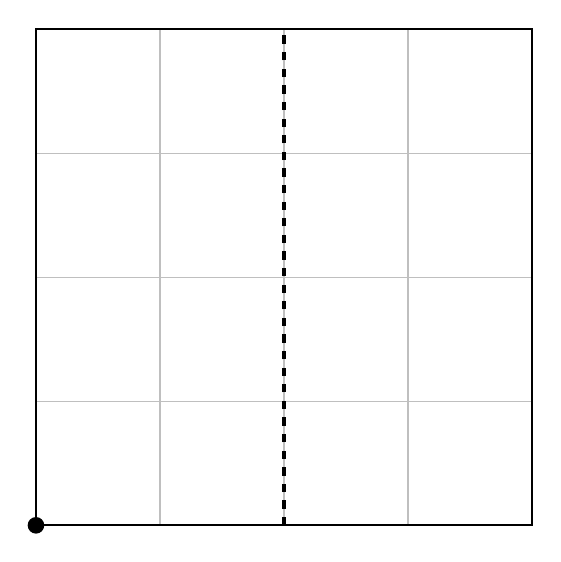
\begin{tikzpicture}[x=.62in,y=.62in]\draw[step=1,black!25](0,0)grid(4,4);\draw[thick](0,0)rectangle(4,4);\draw[dashed,very thick](2,0)--(2,4);\fill(0,0)circle(3pt);\end{tikzpicture}\end{center}
\Problem{6}{These are mirror copies of the wide table. Draw the same straight diagonal, then fold on this dashed wall. Trace the bouncing path and point to its ending corner. Compare it with Problem 5.}
\begin{center}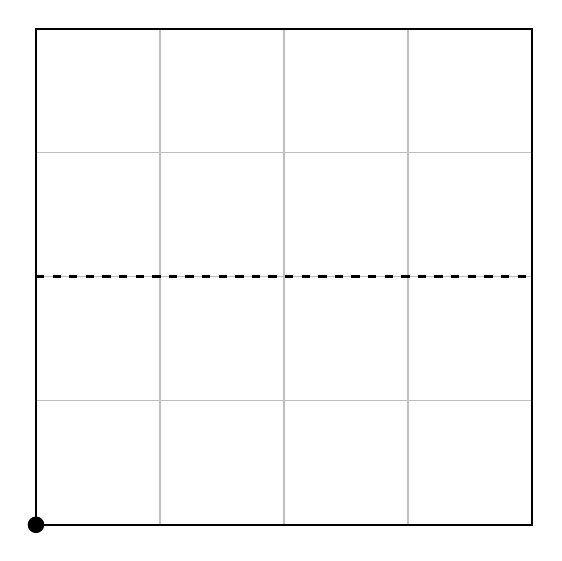
\begin{tikzpicture}[x=.62in,y=.62in]\draw[step=1,black!25](0,0)grid(4,4);\draw[thick](0,0)rectangle(4,4);\draw[dashed,very thick](0,2)--(4,2);\fill(0,0)circle(3pt);\end{tikzpicture}\end{center}

\end{document}
